\section{Bonus : Envoi d'un courrier (3 points)}

Le tableau ci-dessous présente des tarifs d'envoi de courrier de la Poste (en 2009) :

\begin{center}
	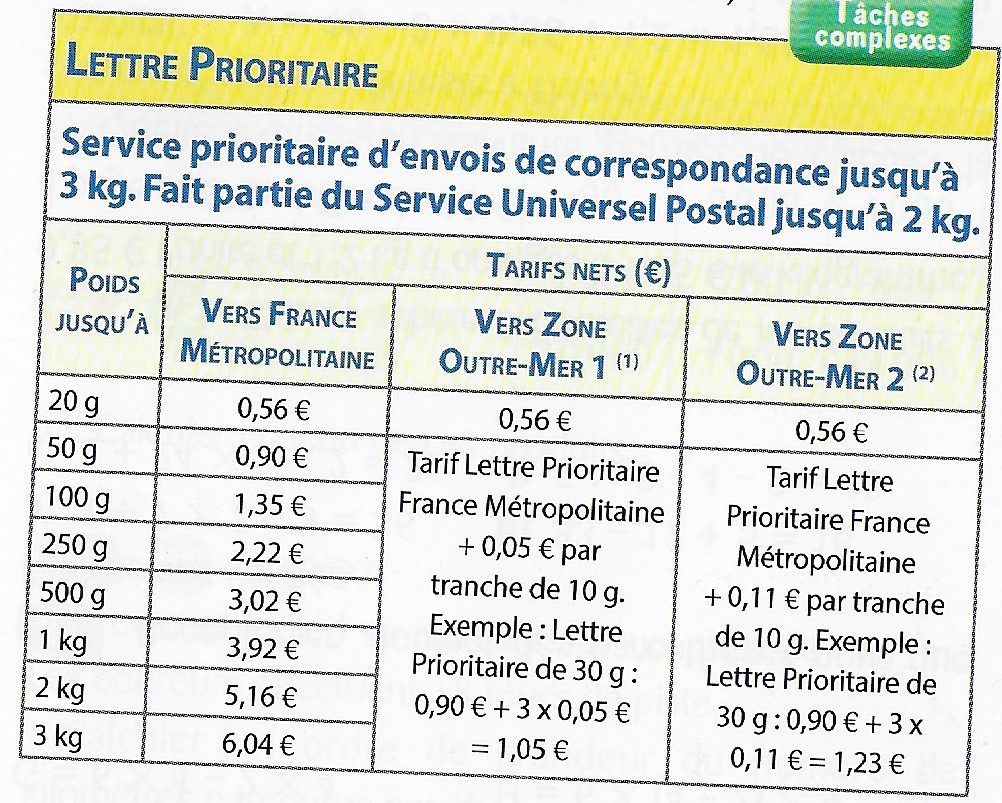
\includegraphics[scale=1.1]{img/poste}
\end{center}

\begin{questions}
	\question[1] Virginie envoie une lettre de 180 g vers la \textbf{Zone Outre-Mer 1}. Vérifier qu'elle va payer \num{3.12} €.
	
	\begin{solution}
		Pour une lettre de 180 g elle devra payer le prix d'une lettre de 250g plus 18 fois 5 centimes.
		
		\begin{equation*}
			\num{2.22} + 18 \times \num{0.05} = \num{3.12}
		\end{equation*}
		
		Elle paiera donc bien \num{3.12} €.
	\end{solution}
	
	\question[1] Cathy envoie une lettre de 2 kg vers la \textbf{Zone Outre-Mer 2}. Combien va-t-elle payer ?
	\begin{solution}
		Pour une lettre de 2 kg elle devra payer \num{5.16} € plus 200 fois 11 centimes.
		
		\begin{equation*}
		\num{5.16} + 200 \times \num{0.11} = \num{27.16}
		\end{equation*}
		
		Elle paiera donc \num{27.16} €.
	\end{solution}
	
	\question[1] Théo poste une lettre pour la \textbf{Zone Outre-Mer 2}, il paye \num{6.32} €. Quelle est la masse maximale de sa lettre ?
	
	\begin{solution}
		Envoyer une lettre de 250 g couterait \num{4.97} € et 500 g couterait \num{8.52} €. Donc la lettre aura une masse comprise entre 250 et 500 grammes.
	\end{solution}
	

	

\end{questions}